\documentclass[12pt]{article}

\usepackage{amsmath, mathtools}
\usepackage{amsfonts}
\usepackage{amssymb}
\usepackage{graphicx}
\usepackage{colortbl}
\usepackage{xr}
\usepackage{hyperref}
\usepackage{longtable}
\usepackage{xfrac}
\usepackage{tabularx}
\usepackage{float}
\usepackage{siunitx}
\usepackage{booktabs}
\usepackage{caption}
\usepackage{pdflscape}
\usepackage{afterpage}

\usepackage[square]{natbib}

%\usepackage{refcheck}

\hypersetup{
    bookmarks=true,         % show bookmarks bar?
    colorlinks=true,       % false: boxed links; true: colored links
    linkcolor=red,          % color of internal links (change box color with linkbordercolor)
    citecolor=green,        % color of links to bibliography
    filecolor=magenta,      % color of file links
    urlcolor=cyan           % color of external links
}

% For easy change of table widths
\newcommand{\colZwidth}{1.0\textwidth}
\newcommand{\colAwidth}{0.13\textwidth}
\newcommand{\colBwidth}{0.82\textwidth}
\newcommand{\colCwidth}{0.1\textwidth}
\newcommand{\colDwidth}{0.05\textwidth}
\newcommand{\colEwidth}{0.8\textwidth}
\newcommand{\colFwidth}{0.17\textwidth}
\newcommand{\colGwidth}{0.5\textwidth}
\newcommand{\colHwidth}{0.28\textwidth}

% Used so that cross-references have a meaningful prefix
\newcounter{defnum} %Definition Number
\newcommand{\dthedefnum}{GD\thedefnum}
\newcommand{\dref}[1]{GD\ref{#1}}
\newcounter{datadefnum} %Datadefinition Number
\newcommand{\ddthedatadefnum}{DD\thedatadefnum}
\newcommand{\ddref}[1]{DD\ref{#1}}
\newcounter{theorynum} %Theory Number
\newcommand{\tthetheorynum}{TM\thetheorynum}
\newcommand{\tref}[1]{TM\ref{#1}}
\newcounter{tablenum} %Table Number
\newcommand{\tbthetablenum}{T\thetablenum}
\newcommand{\tbref}[1]{TB\ref{#1}}
\newcounter{assumpnum} %Assumption Number
\newcommand{\atheassumpnum}{P\theassumpnum}
\newcommand{\aref}[1]{A\ref{#1}}
\newcounter{goalnum} %Goal Number
\newcommand{\gthegoalnum}{P\thegoalnum}
\newcommand{\gsref}[1]{GS\ref{#1}}
\newcounter{instnum} %Instance Number
\newcommand{\itheinstnum}{IM\theinstnum}
\newcommand{\iref}[1]{IM\ref{#1}}
\newcounter{reqnum} %Requirement Number
\newcommand{\rthereqnum}{P\thereqnum}
\newcommand{\rref}[1]{R\ref{#1}}
\newcounter{nfrnum} %NFR Number
\newcommand{\rthenfrnum}{NFR\thenfrnum}
\newcommand{\nfrref}[1]{NFR\ref{#1}}
\newcounter{lcnum} %Likely change number
\newcommand{\lthelcnum}{LC\thelcnum}
\newcommand{\lcref}[1]{LC\ref{#1}}
\newcounter{ucnum} %Likely change number
\newcommand{\ltheucnum}{LC\theucnum}
\newcommand{\ucref}[1]{UC\ref{#1}}

\usepackage{fullpage}

\newcommand{\deftheory}[9][Not Applicable]
{
\newpage
\noindent \rule{\textwidth}{0.5mm}

\paragraph{RefName: } \textbf{#2} \phantomsection 
\label{#2}

\paragraph{Label:} #3 

\noindent \rule{\textwidth}{0.5mm}

\paragraph{Equation:}

#4

\paragraph{Description:}

#5

\paragraph{Notes:}

#6

\paragraph{Source:}

#7

\paragraph{Ref.\ By:}

#8

\paragraph{Preconditions for \hyperref[#2]{#2}:}
\label{#2_precond}

#9

\paragraph{Derivation for \hyperref[#2]{#2}:}
\label{#2_deriv}

#1

\noindent \rule{\textwidth}{0.5mm}

}

\begin{document}


\title{Software Requirements Specification for Retinal Vessel Segmentation System (RVSS)} 
\author{Xinyu Ma}
\date{February 5, 2024}
	
\maketitle

~\newpage

\pagenumbering{roman}

\tableofcontents

~\newpage

\section*{Revision History}

\begin{tabularx}{\textwidth}{p{3cm}p{2cm}X}
\toprule {\bf Date} & {\bf Version} & {\bf Notes}\\
\midrule
02/05/2024 & \;\; 1.0 & Initial Release\\

\bottomrule
\end{tabularx}

~\newpage

\section{Reference Material}

This section records information for easy reference.

\subsection{Table of Units}

Throughout this document SI (Syst\`{e}me International d'Unit\'{e}s) is employed as the unit system.  In addition to the basic units, several derived units are used as described below.  For each unit, the symbol is given followed by a description of the unit and the SI name.
~\newline

\renewcommand{\arraystretch}{1.2}
%\begin{table}[ht]
  \noindent \begin{tabular}{l l l} 
    \toprule		
    \textbf{symbol} & \textbf{unit} & \textbf{SI}\\
    \midrule 
    \si{px} & resolution & pixel\\
    \bottomrule
  \end{tabular}
  %	\caption{Provide a caption}
%\end{table}


Physical units like kilogram ($\si{\kilogram}$) and meter ($\si{\metre}$) are not typically used directly within deep learning models for image segmentation stems from the models' reliance on pixel-level data and abstract feature detection, alongside the practical need for models to generalize across various contexts without being constrained by the specifics of physical measurements. In image segmentation, the input to the model is an array of pixel values. These values do not inherently contain information about physical dimensions or weights. The segmentation process is concerned with classifying each pixel into a category based on features extracted from the image data, irrespective of the physical size or weight of the objects depicted.


\subsection{Table of Symbols}

The table that follows summarizes the symbols used in this document. The choice of symbols was made to be consistent with the image segmentation literature and with existing documentation for retinal vessel segmentation system. The symbols are listed in alphabetical order.

\renewcommand{\arraystretch}{1.2}
\noindent 
\begin{longtable*}{l l} 
    \toprule
    \textbf{symbol} & \textbf{description}\\
    \midrule 
    $\theta$ & CNN Model Parameters\\
    $F_{feature}$ & Feature Extraction Function \\
    $F_{pre}$ & Image preprocess Function\\
    $I$ & retinal image\\ 
    $I_{pre}$ & preprocessed retinal image\\ 
    $I_{seg}$ & segmented retinal binary image\\
    $S_{feature}$ & Feature Maps \\
   
    \bottomrule
\end{longtable*}

\subsection{Abbreviations and Acronyms}

\renewcommand{\arraystretch}{1.2}
\begin{longtable*}{l l} 
  \toprule		
  \textbf{symbol} & \textbf{description}\\
  \midrule
 
  A & Assumption\\
  CLAHE & Contrast Limited Adaptive Histogram Equalization\\
  CNN & Convolution Neural Network\\
  DD & Data Definition\\
  DR & Diabetic Retinopathy
  GD & General Definition\\
  GS & Goal Statement\\
  IM & Instance Model\\
  LC & Likely Change\\
  ML & Machine Learning
  PS & Physical System Description\\
  R & Requirement\\
  RVSS & Retinal Vessel Segmentation System\\ 
  SRS & Software Requirements Specification\\
  TM & Theoretical Model\\
  \bottomrule
\end{longtable*}\\

\newpage

\pagenumbering{arabic}

\section{Introduction}

Information about the structure of the retina’s blood vessels plays a significant role in the recognition and treatment of many illnesses, including age-related macular degeneration, diabetic retinopathy (DR), cardiovascular disease, and glaucoma. However, extracting blood vessels from retinal images is a time-consuming and difficult task. Therefore, a smart system is required that automatically extracts retinal vessels from the raw retinal images and provides them to a 
specialist for diagnosis and treatment. The project aims to use deep learning methods to train a model that can achieve accurate retinal blood vessel segmentation.

The following sections summarize the Software Requirement Specification (SRS) for Retinal Vessel Segmentation System (RVSS). This section includes the purpose of the document, the scope of requirements, the characteristics of the intended reader, and the organization of the document.   


\subsection{Purpose of Document}

The purpose of this document is to provide a detailed overview of the Retinal Vessel Segmentation System (RVSS) outlining its functionality, interface requirements, performance metrics, and constraints. This system is designed to automatically segment retinal vessels from fundus images, aiding in the diagnosis and monitoring of various ocular diseases. This document serves as the basis for the outline design of the system, helping developers quickly understand the framework ideas and implementation functions of the system, and verify whether the system can meet the standards required by users. This facilitates the management of technical documentation and requirements changes, and is also the basis for users and developers to gain a common understanding of software requirements.



\subsection{Scope of Requirements} 

Retinal Vessel Segmentation System (RVSS) is a deep learning-based application intended for use by healthcare professionals to enhance the analysis of retinal images. By accurately segmenting the blood vessel structure of the retina, the system supports the early detection and treatment planning of conditions like diabetic retinopathy, glaucoma, and age-related macular degeneration. 

\subsection{Characteristics of Intended Reader} \label{sec_IntendedReader}

The intended reader should have knowledge of machine learning (ML) and it is highly suggested to have some basic knowledge of computer vision. In machine learning, the intended readers should have an understanding of the process of model training, network architectures, loss functions, supervised learning and unsupervised learning. In computer vision, the intended readers should have knowledge of semantic segmentation. The intended reader should have completed at least one machine learning related courses during their bachelor of Engineering or Science (Computer Science and Software Engineering expected). 


\subsection{Organization of Document}
The rest of the document is organized as follows. Section 3 and Section 4 contain general system description and specific system description respectively. In Section 5, it shows requirement.  


\section{General System Description}

This section provides general information about the system. It identifies the interfaces between the system and its environment, describes the user characteristics and lists the system constraints.

\subsection{System Context}

The system context is shown in Figure \ref{Fig_SystemContext} below. The circles on the left and right represent users who provide input in the specified format required by the retinal segmentation software program and receive output provided by the program. The rectangle represents the retinal segmentation software program itself. The arrows represent data and information transferred between the user and the software program.
\begin{figure}[h!]
\begin{center}
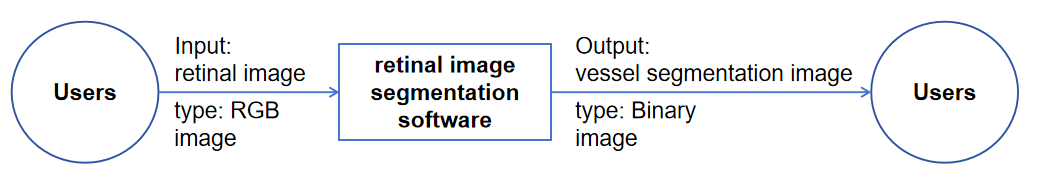
\includegraphics[width=0.7\textwidth]{System Context}
\caption{System Context}
\label{Fig_SystemContext} 
\end{center}
\end{figure}

\begin{itemize}
\item User Responsibilities:
\begin{itemize}
\item \textbf{Data Preparation and Upload}: Users should ensure that the retinal images uploaded to RVSS are of high quality and conform to the system's requirements regarding format, resolution, and size. This includes verifying that the images are correctly focused and free from artifacts that could impair the segmentation process.. 
\item \textbf{Patient Data Confidentiality}: Users are responsible for maintaining the confidentiality of patient data which includes ensuring that patient identifiers are removed or appropriately managed within the system.
\item \textbf{Reporting and Feedback}: Users should report any issues, inaccuracies, or malfunctions experienced while using RVSS to the support team. Providing feedback on system performance and usability can help developers improve the system in future releases.
\item \textbf{Training and Education}: Users should undergo sufficient training to understand how to use RVSS effectively and should keep abreast of any new features or changes to the system.
\item \textbf{Ethical Use}: Since retinal images involve patient privacy, users must ensure that RVSS is used ethically and responsibly, avoiding any abuse that may harm patients or violate privacy rights.
\end{itemize}

\item Software Responsibilities:
\begin{itemize}
\item \textbf{Accurate Segmentation}: RVSS is responsible for accurately segmenting retinal vessels from retinal images. It must utilize advanced algorithms and deep learning models to ensure high accuracy and recall in segmentation, critical for the diagnosis and monitoring of ocular diseases (accuracy$\geq$ 90$\%$,recall$\geq$ 90$\%$). 
\item \textbf{Data Detection}: Detect whether the inputs provided by users satisfy the required system constraints.
\item \textbf{Data Process}: Resize the input images into specified size convert them into grayscale. Then apply contrast limited adaptive histogram equalization (CLAHE) operation on retinal images to increase the contrast of retinal images.
\item \textbf{Model Training}: Train the model and output the vessel segmentation map corresponding to the input image.
\item \textbf{Performance Efficiency}: The system is responsible for processing images and delivering results in a timely manner. Even with large datasets or high-resolution images, the system is essential to support clinical decision-making processes without significant delays (process time $\leq$ 10 seconds).
\item \textbf{Data Security and Patient Privacy}: The system must implement stringent data security measures to protect sensitive patient information. 
\item \textbf{Interoperability}: The system should be capable of integrating smoothly with other healthcare IT systems, such as Electronic Health Records (EHRs) and Picture Archiving and Communication Systems (PACS), facilitating seamless data exchange and workflow integration.
\end{itemize}
\end{itemize}
\subsection{User Characteristics} \label{SecUserCharacteristics}

The end user of the system are divided into two categories, one is those who use the segmentation results for medical analysis, and the other is those who use the segmentation results to study the field of image segmentation. For those who use the segmentation results for medical analysis (e.g., ophthalmologists, radiologists, medical researchers), they are expected to  be familiar with the structure of the retina and they need to understand the biomarkers of some diseases on retinal blood vessels so that they can diagnose related diseases based on vessel structural characteristics such as the vessel length, width, curvature, and bifurcation patterns. For those who use the segmentation results to study the field of image segmentation, they are expected to be familiar with undergraduate level machine learning and know basics about the semantic segmentation. 

\subsection{System Constraints}

System constraints limit the developers’ options in the system design and they identify how the eventual system must fit into the
world. These constraints can impact the design, development, deployment, and usability of the system. Identifying these constraints is crucial for ensuring that the system meets its objectives while operating within these predefined boundaries. Here are key system constraints that apply to RVSS: 
\begin{itemize}
\item \textbf{Hardware Limitations}: The performance and efficiency of RVSS can be constrained by the hardware on which it is deployed. This includes processing power, memory capacity, and storage, which affect the system's ability to process large or high-resolution images quickly. For deep learning tasks, the GPU can accelerate data preprocessing and other non-GPU tasks, and it is recommended to be AMD Ryzen 7 or Intel Core i7. The GPU is used to accelerate the training time of the model, and it is recommended to be NVIDIA RTX 3070 or higher. In addition, since deep learning needs to process a large amount of data, it is recommended to use 32GB RAM to ensure the smooth running of most tasks.

\item  \textbf{Software Compatibility}: RVSS must be compatible with the operating systems and other software tools commonly used in healthcare settings, such as electronic health records systems or diagnostic software. It limits the system's deployment and usability.

\item \textbf{Scalability}: The system must be designed to handle varying loads, from small clinics to large hospitals with thousands of images. Scalability constraints affect how the system architecture is designed to ensure it can grow without significant performance degradation.

\item \textbf{Data Privacy}: Ensuring the confidentiality, integrity, and availability of patient data imposes constraints on how data is processed, stored, and transmitted by RVSS. 
\end{itemize}

\section{Specific System Description}

This section first presents the problem description, which gives a high-level view of the problem to be solved. This is followed by the solution characteristics specification, which presents the assumptions, theories, definitions and finally the instance models of RVSS. 

\subsection{Problem Description} \label{Sec_pd}

Retinal images contain rich retinal blood vessel features \cite{wu2020nfn+,li2020lightweight}. Analyzing the length, width, curvature and other structural characteristics of retinal blood vessels can obtain the clinical and pathological characteristics of many diseases, which is of great significance for the prevention and treatment of these diseases \cite{wu2021scs,wang2020dofe}. For example, the diameter of thin blood vessels and thick blood vessels used for microaneurysm detection are important biomarkers for the diagnosis of diabetic retinopathy \cite{yan2018three}. Retinal blood vessel segmentation is a necessary step to obtain these structural properties. The segmentation results will make subsequent feature extraction and anomaly detection analysis more efficient and accurate. Due to the complex tree structure of retinal blood vessels, artificial retinal blood vessel segmentation has various problems such as error-prone, time-consuming, and tedious \cite{jin2019dunet,oliveira2018retinal}. The project is intended to introduce deep learning into the field of medical image processing, using deep learning methods to achieve automatic segmentation of retinal blood vessels, thereby helping doctors analyze complex retinal images.

\subsubsection{Terminology and  Definitions}

This subsection provides a list of terms that are used in the subsequent sections and their meaning, with the purpose of reducing ambiguity and making it easier to correctly understand the requirements:

\begin{itemize}

\item Fundus Camera: Fundus Camera is an analytical instrument used in the field of clinical medicine and can be used to examine the vitreous body, retina, choroid, etc.
\item Retinal Image: Retinal Image is a digital image of the back of your eye obtained by fundus camera. It shows the retina (where light and images hit), the optic disc (a spot on the retina that holds the optic nerve, which sends information to the brain), and blood vessels.
\item Binary Image: Binary Image is one that consists of pixels that can have one of exactly two colors, usually black and white. 
\item RGB Image: RGB Image is a bitmap image holding RGB color values in three image channels.
\item Semantic Segmentation: Semantic segmentation is a deep learning algorithm that associates a label or category with every pixel in an image. It is used to recognize a collection of pixels that form distinct categories.
\item Supervised Learning: Supervised Learning is a category of machine learning that uses labeled datasets to train algorithms to predict outcomes and recognize patterns.
\item Loss Function: Loss Function is a mathematical function that quantifies the difference between predicted and actual values in a machine learning model.
\item Classifier: Classifier in machine learning is an algorithm that automatically orders or categorizes data into one or more of a set of classes based on some set of features.
\item Binary Classifiers: Binary Classifiers are used when there are only two possible classes. For example, an email classifier might be designed to detect spam and non-spam emails.
\item Accuracy: Accuracy is a metric that measures how often a machine learning model correctly predicts the outcome. 
\item Sensitivity: Sensitivity is a measure of how well a machine learning model can detect positive instances. In other words, sensitivity measures the proportion of actual positives that are correctly identified as such.
\item Specificity: Specificity measures the proportion of true negatives that are correctly identified by the model.
\end{itemize}

\subsubsection{Physical System Description} \label{sec_phySystDescrip}

The physical system of RVSS involves the integration of hardware and software components designed to accurately segment retinal vessels from fundus images. The following is the physical system description for RVSS, detailing its elements, properties, and interactions. The physical system of RVSS, as shown in Figure \ref{Fig_PhysicalSystem},
includes the following elements:

\begin{figure}[h!]
\begin{center}
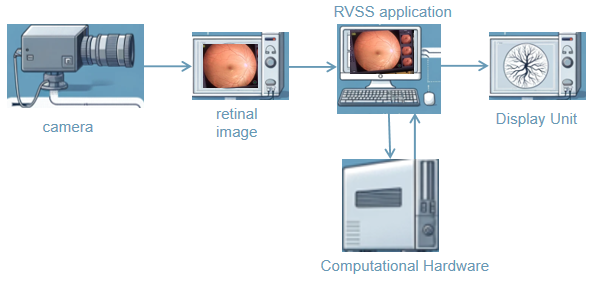
\includegraphics[width=0.60\textwidth]{physical system}
\caption{Physical System of RVSS}
\label{Fig_PhysicalSystem} 
\end{center}
\end{figure}

\begin{itemize}

\item[PS1:] Input Device (Camera/Scanner): Properties include resolution, sensitivity and dynamic range.

\item[PS2:] Retinal Images: Properties include image resolution, bit depth and field of view.

\item[PS3:] Computational Hardware: Properties include processor speed, RAM size and storage capacity.

\item[PS4:] Software (RVSS Application): Properties include compatibility and user interface design.

\item[PS5:] Display Unit (Monitor): Properties include resolution, size and color depth.

\end{itemize}

The physical description of RVSS can also include interactions of the elements: i) the interactions between the elements and their physical environment; ii) the interactions between elements; and, iii) the initial or boundary conditions.

Interactions between elements and their physical environment include:
\begin{itemize}

\item The input device (PS1) captures retinal images (PS2) in a controlled lighting environment to ensure image quality.

\item Computational hardware (PS3) operates within an environment with sufficient cooling to prevent overheating and maintain performance.

\end{itemize}

Interactions between elements include:
\begin{itemize}

\item Retinal images (PS2) are transferred from the input device (PS1) to the Software (RVSS Application) (PS4) for processing.

\item The Software (RVSS Application) (PS4) installed on the computational hardware (PS3) analyzes the retinal images (PS2) to segment retinal vessels.

\item Segmentation result are displayed on the display unit (PS5), allowing for user interaction and interpretation.
\end{itemize}

The initial or boundary conditions include:
\begin{itemize}

\item The computational hardware (PS3) must have the requisite specifications to run the Software (RVSS Application) (PS4) effectively, including processing power and memory.
\end{itemize}

\subsubsection{Goal Statements}
The goal statements of a Retinal Vessel Segmentation System (RVSS) articulate the primary objectives that the system aims to achieve. These statements provide criteria for sufficient completeness of a requirements specification and for requirements pertinence. 
The following are the goal statements for RVSS:

\noindent Given the inputs, the goal statement is:

\begin{itemize}

\item[GS\refstepcounter{goalnum}\thegoalnum \label{G_meaningfulLabel}:] \textbf{Accurate Segmentation}: To provide highly accurate and precise (accuracy $\leq$ 90$\%$) segmentation of retinal vessels from retinal images, enabling detailed analysis of the retinal vascular structure . 


\item[GS\refstepcounter{goalnum}\thegoalnum \label{G_meaningfulLabel}:] \textbf{Enhanced Diagnostic Support}: To aid healthcare professionals in the diagnosis and monitoring of ocular diseases, such as diabetic retinopathy, glaucoma, and age-related macular degeneration, by offering detailed visualizations of retinal blood vessels. For each given retinal RGB image input, display the corresponding vessel segmentation image, i.e., a binary image, the vessel part is represented by white pixels, and the other parts are represented by black pixels.

\item[GS\refstepcounter{goalnum}\thegoalnum 
\label{G_meaningfulLabel}:] \textbf{Usability}: To offer an intuitive and user-friendly interface (each option in the software is clearly stated) that enables healthcare professionals, regardless of their technical expertise, to easily operate the RVSS and interpret its outputs. 

\end{itemize}

\subsection{Solution Characteristics Specification}
This section specifies the information in the solution domain of the system to be developed. The purpose of this section is to reduce the problem into one expressed in mathematical terms. This section presents the solution characteristics by successively refining models. It starts with the abstract/general Theoretical Models (TMs) and refines them to the concrete/specific Instance Models (IMs).

The Theoretical Models (TMs) for the Retinal Vessel Segmentation System (RVSS) provide the foundational theoretical framework on which the system's algorithms and processes are built. These models describe the abstract principles that underpin the methods used for segmenting blood vessels from retinal images. Here are the TMs for RVSS:

\begin{itemize}

\item[TM1:]Image Segmentation Model:  Given an image $I$, segmentation partitions $I$ into $n$ segments $\{S_1,S_2,...,S_n\}$, such that $\bigcup_{i=1}^{n}S_i = I$ and $S_i \cup S_j = \emptyset$ for all $i \neq j$where each $S_i$ represents a segment of the image sharing common characteristics.

\item[TM2:]{Convolution Neural Networks (CNN) for Image Analysis}:A CNN function $F_{CNN}$ maps an input image $I$ to an output $O$, where $O=F_{CNN}(I,\theta)$ and $\theta$ represents the parameters of the CNN. The function $F_{CNN}$ includes convolution operations that filter $I$ through multiple layers to extract features relevant for segmentation.

\item[TM3:]Feature Extraction and Representation:  Given an image $I$, feature extraction can be represented as a function $F_{feature}$ that maps $I$ to a feature space $S_{feature}$, where $S_{feature} = F_{feature}(I)$. This function identifies and isolates features relevant to retinal vessels.

\end{itemize}

The General Definitions (GDs) of RVSS include Convolutional Operation which is derived from TM2. Given an image matrix $I$ and a filter matrix $FI$, the convolution operation $C(I,FI)$ produces a feature map $M$. 

The Instance Models (IMs) of RVSS include Retinal Vessel Segmentation Using CNN which is derived from TM2. The mathematical representation of IM1 is:
\begin{itemize}
    \item Input: a preprocessed retinal image $I_{retinal}$.
    \item Output: a binary segmented image $I_segmentation$,where pixels belonging to retinal vessels are marked as 1 (vessel) and others as 0 (background).
    \item Process: $I_segmentation = F_{CNN} (I_{retinal}, \theta)$, where $\theta$ represents the learned parameters of the $CNN$.
\end{itemize}

The Assumptions (A) includes the retinal images are preprocessed to have uniform dimensions and contrast levels before segmentation and the retinal vessels and background have sufficient contrast to be distinguished by the $CNN$.

\subsubsection{Types}
Defining types can make the document easier to understand. The following are the types used in this SRS document.
\begin{itemize}
    \item Image Type: For RVSS, image types might include raw retinal images, preprocessed images, and segmented images, with formats such as JPEG, PNG, or TIFF.
    \item Model Type: Defines the various kinds of models used within RVSS, including CNNs for image analysis, and other machine learning models. Model types may distinguish between architectures (e.g., U-Net, VGG16) or purposes (e.g., image segmentation, image classification).
     \item Feature Type: The categories of features extracted from images for analysis, such as texture features, or shape features.
     \item Output Type: The types of outputs generated by RVSS, i.e., binary segmented images, probability maps indicating the likelihood of vessel presence.

\end{itemize}





\subsection{Modelling Decisions}
\subsubsection{Assumptions} \label{sec_assumpt}
The assumptions are a refinement of the scope. This section simplifies the original problem and helps in developing the theoretical model by filling in the missing information for the physical system. The numbers given in the square brackets refer to the theoretical model [TM], general definition [GD], data definition [DD], instance model [IM], or likely change [LC], in which the respective assumption is used.
 

\begin{itemize}

\item[A\refstepcounter{assumpnum}\theassumpnum \label{A_1}:] High-Quality Input Images, RVSS assumes that the input retinal images are of high quality, with adequate resolution and clarity to enable accurate segmentation of retinal vessels, e.g., the retinal vessels and background have sufficient contrast to be distinguished by the $CNN$. [\tref{TM_1}, \ddref{dd_1}, \iref{im_2}] 

\item[A\refstepcounter{assumpnum}\theassumpnum \label{A_2}:] Standardized Image Formats, RVSS assumes that all input images are provided in standardized digital formats (e.g., JPEG, PNG, TIFF) compatible with the system. \tref{TM_1}, \ddref{dd_1}, \iref{im_2}] 

\item[A\refstepcounter{assumpnum}\theassumpnum \label{A_3}:] Preprocessed Data, RVSS assumes that input images require preprocessing, such as normalization and contrast enhancement, to have uniform dimensions and contrast levels before segmentation. [\tref{TM_2}, \ddref{dd_2}, \iref{im_1}, \iref{im_2}, \iref{im_3}] 


\item[A\refstepcounter{assumpnum}\theassumpnum \label{A_4}:]Stable Operating Environment, RVSS assumes that the software operates in a stable and controlled computing environment. [\tref{TM_2}, \tref{TM_3}, \ddref{dd_3}, \dref{GD_1}, \dref{GD_2},\dref{GD_3},\iref{im_1}, \iref{im_3}] 


\end{itemize}



\subsubsection{Theoretical Models}\label{sec_theoretical}

Theoretical models are sets of abstract mathematical equations or axioms for solving the problem described in Section ``Physical System Description''(Section~\ref{sec_phySystDescrip}).This section focuses on the general equations and laws that Retinal Vessel segmentation is based on.


~\newline

\noindent
\begin{minipage}{\textwidth}
\renewcommand*{\arraystretch}{1.5}
\begin{tabular}{| p{\colAwidth} | p{\colBwidth}|}
  \hline
  \rowcolor[gray]{0.9}
  Number& TM\refstepcounter{theorynum}\thetheorynum \label{TM_1}\\
  \hline
  Label& \bf Image Segmentation Model\\
  \hline
  Equation &
    Input: image $I$\\
    &Output: $\{S_1,S_2,...,S_n\}$, where$\bigcup_{i=1}^{n}S_i = I$, $S_i \cup S_j = \emptyset$ for all $i \neq j$ \\ 
  \hline
  Description
    & This model outlines the theory behind segmenting digital images into meaningful components. It is the process of dividing an image into different regions based on the characteristics of pixels to identify objects or boundaries to simplify an image and more efficiently analyze it.
\\
  & Given an image $I$, segmentation partitions $I$ into $n$ segments $\{S_1,S_2,...,S_n\}$, where each $S_i$ represents a segment of the image sharing common characteristics.\\ 

  \hline
  Notes & None\\
  \hline
  Sources& \url{https://ai.stanford.edu/~syyeung/cvweb/index.html} \\
  \hline
  Ref.\ By &  \iref{im_2}\\
  \hline
\end{tabular}
\end{minipage}\\


~\newline

\noindent
\begin{minipage}{\textwidth}
\renewcommand*{\arraystretch}{1.5}
\begin{tabular}{| p{\colAwidth} | p{\colBwidth}|}
  \hline
  \rowcolor[gray]{0.9}
  Number& TM\refstepcounter{theorynum}\thetheorynum \label{TM_2}\\
  \hline
  Label& \bf Convolution Neural Networks (CNN) for Image Analysis\\
  \hline
  Equation &
    $O=F_{CNN}(I,\theta)$ \\ 
  \hline
  Description
    & This model explains the use of CNN in analyzing and interpreting images. CNNs are deep learning algorithms that can take an input image, assign importance to various aspects of the image under different perspectives, and differentiate between these aspects to achieve tasks such as image segmentation.  \\
  
   & $F_{CNN}$ is a  CNN function that maps an input image $I$ to an output $O$. The function $F_{CNN}$ includes convolution operations that filter $I$ through multiple layers to extract features relevant for segmentation.\\
   
   & $\theta$ represents the parameters of $CNN$.  \\
  
  \hline
  Notes & Understand image segmentation using CNN and explore how to create, train, and evaluate neural networks for image segmentation tasks. \\
  \hline
  Sources& \url{https://www.analyticsvidhya.com/blog/2021/06/image-processing-using-cnn-a-beginners-guide/} \\
  \hline
  Ref.\ By &  \iref{im_1} \\
  \hline
\end{tabular}
\end{minipage}\\
~\newline




\noindent
\begin{minipage}{\textwidth}
\renewcommand*{\arraystretch}{1.5}
\begin{tabular}{| p{\colAwidth} | p{\colBwidth}|}
  \hline
  \rowcolor[gray]{0.9}
  Number& TM\refstepcounter{theorynum}\thetheorynum \label{TM_3}\\
  \hline
  Label& \bf Feature Extraction and Representation\\
  \hline
  Equation &
    $S_{feature} = F_{feature}(I)$ \\ 
  \hline
  Description
    & This model describes the process of extracting features from images, which is crucial for understanding the content of the image and for tasks like segmentation. It refers to the process of transforming raw data into numerical features that can be processed while preserving the information in the original data set. Feature extraction in RVSS involves identifying characteristics of retinal vessels, such as their shape, size, and orientation, which distinguish them from the background. \\
  
   & $I$ is the input image.\\
   
   & $F_{feature}$ is the function of feature extraction that maps $I$ to a feature space $S_{feature}$.\\
   
   &This function identifies and isolates features relevant to retinal vessels.\\

  \hline
  Notes & None \\
  \hline
  Sources& \url{https://www.mathworks.com/discovery/feature-extraction.html} \\
  \hline
  Ref.\ By & \iref{im_3} \\
  \hline
\end{tabular}
\end{minipage}\\
~\newline



\subsubsection{General Definitions}\label{sec_gendef}
General Definitions (GDs) are a refinement of one or more TMs, and/or of other GDs. This section collects the laws and equations that will be used in building the instance models.


~\newline

\noindent
\begin{minipage}{\textwidth}
\renewcommand*{\arraystretch}{1.5}
\begin{tabular}{| p{\colAwidth} | p{\colBwidth}|}
  \hline
  \rowcolor[gray]{0.9}
  Number& GD\refstepcounter{defnum}\thedefnum \label{GD_1}\\
  \hline
  Label& \bf Convolution Layer Calculation\\
  \hline
  Equation &
    $ N=\frac{W - F + 2P}{S} +1$ \\ 
  \hline
  Description
    & The Convolution Layer contains units whose receptive fields cover a patch of the previous layer.
\\
  & $W$ is the size of the input image.\\ 
  & $F$ is the size of the convolution kernel. \\ 
  & $P$ is the size of the padding. \\ 
  & $S$ is the length of the stride. \\ 
  \hline
  Notes & The Convolution layer is part of the network architecture used for model training. \\
  \hline
  Sources& \url{https://en.wikipedia.org/wiki/Convolutional_neural_network} \\
  \hline
  Ref.\ By &  \tref{TM_2}, \iref{im_1}\\
  \hline
\end{tabular}
\end{minipage}\\

~\newline
\noindent
\begin{minipage}{\textwidth}
\renewcommand*{\arraystretch}{1.5}
\begin{tabular}{| p{\colAwidth} | p{\colBwidth}|}
  \hline
  \rowcolor[gray]{0.9}
  Number& GD\refstepcounter{defnum}\thedefnum \label{GD_2}\\
  \hline
  Label& \bf Transposed Convolution Layer Calculation\\
  \hline
  Equation &
    $ TC=S_{TC}(W_{TC}-1)+2P_{TC}-F_{TC}+2$ \\ 
  \hline
  Description
    & The transposed Convolution layer is an upsampling layer that generates the output feature map greater than the input feature map.\\
  & $W_{TC}$ is the size of the input image.\\ 
  & $F_{TC}$ is the size of the convolution kernel. \\ 
  & $P_{TC}$ is the size of the padding. \\ 
  & $S_{TC}$ is the length of the stride. \\ 
  \hline
  Notes & The Transposed Convolution Layer is part of the network architecture used for model training. \\
  \hline
  Sources& \url{https://d2l.ai/chapter_computer-vision/transposed-conv.html} \\
  \hline
  Ref.\ By &  \tref{TM_2}, \iref{im_1}\\
  \hline
\end{tabular}
\end{minipage}\\



~\newline
\noindent
\begin{minipage}{\textwidth}
\renewcommand*{\arraystretch}{1.5}
\begin{tabular}{| p{\colAwidth} | p{\colBwidth}|}
  \hline
  \rowcolor[gray]{0.9}
  Number& GD\refstepcounter{defnum}\thedefnum \label{GD_3}\\
  \hline
  Label& \bf Loss Function\\
  \hline
  Equation &
    $ Loss = |Y_{pred} – Y_{actual}|$ \\ 
  \hline
  Description
    & The loss function is a mathematical function that quantifies the difference between predicted and actual values in a machine learning model. It measures the model’s performance and guides the optimization process by providing feedback on how well it fits the data. If the model predictions are closer to the actual values the loss will be minimum and if the predictions are totally away from the original values the loss value will be the maximum.\\
  & $Y_{pred}$ is the predicted value.\\ 
  & $Y_{actual}$ is the real value. \\ 

  \hline
  Notes & On the basis of the loss value, the model can be updated until getting the best result. \\
  \hline
  Sources& \url{https://www.analyticsvidhya.com/blog/2022/06/understanding-loss-function-in-deep-learning/} \\
  \hline
  Ref.\ By &  \tref{TM_2}, \iref{im_1}\\
  \hline
\end{tabular}
\end{minipage}\\



\subsubsection{Data Definitions}\label{sec_datadef}


The Data Definitions are definitions of symbols and equations that are given for the problem. This section collects and defines all the data needed to build the instance models. The dimension of each quantity is also given.  

~\newline


\noindent
\begin{minipage}{\textwidth}
\renewcommand*{\arraystretch}{1.5}
\begin{tabular}{| p{\colAwidth} | p{\colBwidth}|}
\hline
\rowcolor[gray]{0.9}
Number& DD\refstepcounter{datadefnum}\thedatadefnum \label{dd_1}\\
\hline
Label& \bf Data Definition of retinal image $I$\\
\hline
Symbol & $I$ \\
\hline
% Units& $Mt^{-3}$\\
% \hline
  SI Units &NA\\
  \hline
  Equation&NA \\
  \hline
  Description & Retinal images are high-resolution photographs of the interior surface of the eye, including the retina, optic disc, and blood vessels. These images are captured using specialized fundus camera. In RVSS, retinal images serve as the primary input data for the system.
\\
  \hline
  Sources&\url{https://www.webmd.com/eye-health/what-is-retinal-imaging} \\
  \hline
  Ref.\ By & \tref{TM_1}, \ddref{dd_2}, \ddref{dd_3}, \iref{im_2}\\
  \hline
\end{tabular} \\
\end{minipage}\\

~\newline


\noindent
\begin{minipage}{\textwidth}
\renewcommand*{\arraystretch}{1.5}
\begin{tabular}{| p{\colAwidth} | p{\colBwidth}|}
\hline
\rowcolor[gray]{0.9}
Number& DD\refstepcounter{datadefnum}\thedatadefnum \label{dd_2}\\
\hline
Label& \bf Data Definition of preprocessed images \\
\hline
Symbol &$I_{pre}$\\
\hline
% Units& $Mt^{-3}$\\
% \hline
  SI Units & NA\\
  \hline
  Equation& $I_{pre} = F_{pre}(I)$ \\
  \hline
  Description & This preprocessing step ensures that the images are in a consistent format and condition for effective segmentation. \\
  
  &$F_{pre}$ represents the preprocessing methods, and it includes normalization of intensity levels, contrast enhancement, resizing, noise reduction, and CLAHE. \\
  
  &$I$ is \iref{dd_1} which represents the retinal image. \\
  \hline
  Sources& ~\cite{khandouzi2022retinal} \\
  \hline
  Ref.\ By & \tref{TM_2}, \iref{im_1}, \iref{im_3}\\
  \hline
\end{tabular} \\
\end{minipage}\\

~\newline


\noindent
\begin{minipage}{\textwidth}
\renewcommand*{\arraystretch}{1.5}
\begin{tabular}{| p{\colAwidth} | p{\colBwidth}|}
\hline
\rowcolor[gray]{0.9}
Number& DD\refstepcounter{datadefnum}\thedatadefnum \label{dd_3}\\
\hline
Label& \bf Data Definition of Segmented Images \\
\hline
Symbol &$I_{seg}$\\
\hline
% Units& $Mt^{-3}$\\
% \hline
  SI Units & NA\\
  \hline
  Equation&$I_{seg} = f_{CNN}(I,\theta)$ \\
  \hline
  Description & Segmented images $I_{seg}$ are the output of RVSS, where the retinal vessels have been identified and delineated from the rest of the retina and background. These images typically represent vessels as distinct entities, often marked in binary format (e.g., vessels as 1, background as 0).\\
  

  \hline
  Sources& ~\cite{long2015fully} \\
  \hline
  Ref.\ By & \tref{TM_2}, \iref{im_1}\\
  \hline
\end{tabular} \\
\end{minipage}\\

~\newline


\noindent
\begin{minipage}{\textwidth}
\renewcommand*{\arraystretch}{1.5}
\begin{tabular}{| p{\colAwidth} | p{\colBwidth}|}
\hline
\rowcolor[gray]{0.9}
Number& DD\refstepcounter{datadefnum}\thedatadefnum \label{dd_4}\\
\hline
Label& \bf Data Definition of CNN Model Parameters\\
\hline
Symbol &$\theta$\\
\hline
% Units& $Mt^{-3}$\\
% \hline
  SI Units & NA\\
  \hline
  Equation&NA \\
  \hline
  Description & It consist of the weights and biases of the convolutional neural network used in RVSS for image segmentation. These parameters are learned during the training process and determine how the $CNN$ responds to different features in the retinal images to achieve accurate segmentation\\


  \hline
  Sources& ~\url{https://cs231n.github.io/convolutional-networks/} \\
  \hline
  Ref.\ By & \tref{TM_2}, \iref{im_1}\\
  \hline
\end{tabular} \\
\end{minipage}\\

~\newline


\noindent
\begin{minipage}{\textwidth}
\renewcommand*{\arraystretch}{1.5}
\begin{tabular}{| p{\colAwidth} | p{\colBwidth}|}
\hline
\rowcolor[gray]{0.9}
Number& DD\refstepcounter{datadefnum}\thedatadefnum \label{dd_5}\\
\hline
Label& \bf Data Definition of Feature Maps\\
\hline
Symbol &$S_{feature}$\\
\hline
% Units& $Mt^{-3}$\\
% \hline
  SI Units & NA\\
  \hline
  Equation& NA\\
  \hline
  Description &  Feature maps represent the presence or absence of specific features at different spatial locations in the input data. In RVSS, feature maps highlight specific features of the retinal images that are relevant for identifying retinal vessels.\\
  
  \hline
  Sources& \url{https://medium.com/@saba99/feature-map-35ba7e6c689e} \\
  \hline
  Ref.\ By & \tref{TM_3}, \iref{im_3}\\
  \hline
\end{tabular} \\
\end{minipage}\\

~\newline



\subsubsection{Instance Models} \label{sec_instance}    

This section transforms the problem defined in Section~\ref{Sec_pd} into one which is expressed in mathematical terms. It uses concrete symbols defined in Section~\ref{sec_datadef} to replace the abstract symbols in the models identified in Sections~\ref{sec_theoretical}.


~\newline

%Instance Model 1
\noindent
\begin{minipage}{\textwidth}
\renewcommand*{\arraystretch}{1.5}
\begin{tabular}{| p{\colAwidth} | p{\colBwidth}|}
  \hline
  \rowcolor[gray]{0.9}
  Number& IM\refstepcounter{instnum}\theinstnum \label{im_1}\\
  \hline
  Label& \bf Retinal Vessel Segmentation Using CNN\\
  \hline
  Input&  A preprocessed retinal image $I_{pre}$ (DD2) \\
  \hline
  Output& A binary segmented image $I_{seg}$ (DD3)\\
  \hline
  Description
  & The IM1 implements CNN designed for the retinal vessels segmentation task. The model utilizes a sequence of convolution layer, pooling, and activation layers to process the input images, extract relevant features, and output a segmented image by transposed convolution layer.\\
  &$I_{seg} = F_{CNN}(I_{pre},\theta)$, where $\theta$ represents the learned parameters of the CNN.\\
  &In $I_{seg}$, pixels belong to retinal vessels are marked as 1 (vessel) and others as 0 (background)\\
  \hline
  Sources& \url{https://oden.io/glossary/model-training/} \\
  \hline
  Ref.\ By & None\\
  \hline
\end{tabular}
\end{minipage}\\

~\newline

\noindent
\begin{minipage}{\textwidth}
\renewcommand*{\arraystretch}{1.5}
\begin{tabular}{| p{\colAwidth} | p{\colBwidth}|}
  \hline
  \rowcolor[gray]{0.9}
  Number& IM\refstepcounter{instnum}\theinstnum \label{im_2}\\
  \hline
  Label& \bf Preprocessing of Retinal Images\\
  \hline
  Input& Raw retinal image $I$ (DD1)\\
  \hline
  Output&  Preprocessed retinal image $I_{pre}$ (DD2)\\
  \hline
  Description
  &The IM2 outlines the preprocessing steps applied to retinal images before retinal vessel segmentation using CNN (IM1). IM2 aims to enhance image quality, normalize image characteristics, and prepare the images for efficient analysis by the CNN.\\
  
  \hline
  Sources& \cite{pal2016preprocessing} \\
  \hline
  Ref.\ By & \iref{im_1}\\
  \hline
\end{tabular}
\end{minipage}\\

~\newline
\noindent
\begin{minipage}{\textwidth}
\renewcommand*{\arraystretch}{1.5}
\begin{tabular}{| p{\colAwidth} | p{\colBwidth}|}
  \hline
  \rowcolor[gray]{0.9}
  Number& IM\refstepcounter{instnum}\theinstnum \label{im_3}\\
  \hline
  Label& \bf Feature Extraction for Blood Vessel Identification\\
  \hline
  Input& Preprocessed retinal image $I_{pre}$ (DD2)\\
  \hline
  Output& Feature map $S_{feature}$ (DD5) highlighting blood vessel-specific characteristics.\\
  \hline
  Description
  & $S_{feature}=ExtractFeatures(I_{pre})$ The IM3 describes the extraction of features specific to retinal vessels (e.g., linearity, width, branching patterns) from the preprocessed retinal images. These features are critical for distinguishing blood vessels from the retinal background and for improving the segmentation performance of the CNN.\\
  
  \hline
  Sources& \cite{jogin2018feature}\\
  \hline
  Ref.\ By & \iref{im_1}\\
  \hline
\end{tabular}
\end{minipage}\\

~\newline

\subsubsection{Input Data Constraints} \label{sec_DataConstraints}   

Table~\ref{TblInputVar} shows the data constraints on the input variables. The column for physical constraints gives the physical limitations on the range of values that can be taken by the variable.  The column for software constraints restricts the range of inputs to reasonable values. The software constraints will be helpful in the design stage for picking suitable algorithms. The constraints are conservative, to give the user of the model the flexibility to experiment with unusual situations. The column of typical values is intended to provide a feel for a common scenario. The uncertainty column provides an estimate of the confidence with which the physical quantities can be measured. This information would be part of the input if one were performing an uncertainty quantification exercise.

\begin{table}[!h]
  \caption{Input Variables} \label{TblInputVar}
  \renewcommand{\arraystretch}{1.2}
\noindent \begin{longtable*}{l l l l c} 
  \toprule
  \textbf{Var} & \textbf{Physical Constraints} & \textbf{Software Constraints} &
                             \textbf{Typical Value} & \textbf{Uncertainty}\\
  \midrule 

  $I$ & $Resolution>500*500$ & JPEG, PNG, TIFF & $584*565$ JPEG & -
  \\
  \bottomrule
\end{longtable*}
\end{table}

\subsubsection{Properties of a Correct Solution} \label{sec_CorrectSolution}

\noindent
A correct solution must exhibit fill in the details. These properties are in addition to the stated requirements.  Table~\ref{TblOutputVar} shows the data constraints on the input variables. 

\begin{table}[!h]
\caption{Output Variables} \label{TblOutputVar}
\renewcommand{\arraystretch}{1.2}
\noindent \begin{longtable*}{l l} 
  \toprule
  \textbf{Var} & \textbf{Physical Constraints} \\
  \midrule 
  $I_{seg}$ & Resolution($I_{seg}$) = Resolution($I$)
  \\
  \bottomrule
\end{longtable*}
\end{table}

\section{Requirements}

The requirements refine the goal statement.  They will make heavy use of references to the instance models. This section provides the functional requirements, the business tasks that the software is expected to complete, and the nonfunctional requirements, the qualities that the software is expected to exhibit.

\subsection{Functional Requirements}

\noindent 

\begin{itemize}

\item[R\refstepcounter{reqnum}\thereqnum \label{R_1}:]  The system shall allow users to upload retinal images in specified formats (e.g., JPEG, PNG, TIFF).
\item[R\refstepcounter{reqnum}\thereqnum \label{R_2}:]
The system shall automatically preprocess images for segmentation, including normalization, contrast adjustment, CLAHE or noise reduction.(from \iref{im_2}).

\item[R\refstepcounter{reqnum}\thereqnum \label{R_3}:] The system shall segment retinal vessels from preprocessed retinal images using deep learning algorithms (from \iref{im_1}).

\item[R\refstepcounter{reqnum}\thereqnum \label{R_4}:] The system shall generate results including the segmentation outcomes and metrics (e.g., accuracy, sensitivity, specificity) .

\end{itemize}


\subsection{Nonfunctional Requirements}


\noindent 

\begin{itemize}

\item[NFR\refstepcounter{nfrnum}\thenfrnum \label{NFR_Accuracy}:]
  \textbf{Accuracy} The segmentation accuracy of the system shall meet or exceed specified benchmarks (Accuracy $\leq$ 90$\%$), with a high true positive rate for vessel segmentation.
\item[NFR\refstepcounter{nfrnum}\thenfrnum \label{NFR_Usability}:] \textbf{Usability} The system offer an intuitive graphical user interface that can be used with minimal training and it can be used within simple steps.

\item[NFR\refstepcounter{nfrnum}\thenfrnum \label{NFR_Performance}:] \textbf{Performance} The system process images and return segmentation results within a specified time frame (e.g., less than 5 seconds for standard resolution images).

\item[NFR\refstepcounter{nfrnum}\thenfrnum \label{NFR_Compatibility}:] \textbf{Compatibility} The system should be compatible with standard operating systems used in healthcare environments, such as Windows and MacOS.

\item[NFR\refstepcounter{nfrnum}\thenfrnum \label{NFR_Compatibility}:] \textbf{Maintainability} The system should be designed to facilitate easy updates and maintenance, e.g., algorithm improvements.

\end{itemize}

\subsection{Rationale}
Rationale should be provided for scope decisions, modelling decisions, assumptions and typical values.

In scope decisions, focusing on functionalities like image upload, image preprocessing, and image segmentation ensures that development resources are concentrated on achieving high accuracy in blood vessel segmentation, which is critical for diagnostic purposes. Besides, limit the scope to retinal vessel segmentation without investigating comprehensive disease diagnostic analysis allows the segmentation algorithm to be specifically optimized which ensure that the system excels in the accuracy of vessel segmentation.

In modelling decisions, choose CNN for image analysis is based on their proven success in image-related tasks, particularly in medical imaging, especially its ability to extract features from images aligns with the need for detailed vessel structure recognition. 

In assumptions, high-quality input images acknowledges the fundamental dependency of machine learning models on data quality for achieving high accuracy, guiding users to ensure optimal imaging tasks. 

Typical values for luminance and contrast provide benchmarks for preprocessing algorithms, ensuring that images are optimized for segmentation without losing critical information.


\section{Likely Changes}    

\noindent 
\begin{itemize}

\item[LC\refstepcounter{lcnum}\thelcnum\label{LC_1}:] Expansion of Image Formats (Related to \aref{A_2}). RVSS may need to support additional image formats beyond JPEG, PNG, and TIFF, due to the emergence of new imaging technologies or standards in retinal imaging.


\item[LC\refstepcounter{lcnum}\thelcnum\label{LC_2}:]  Algorithmic Improvements for Accuracy. Continuous improvements and updates to the segmentation algorithms will be necessary to enhance accuracy, such as network architecture and loss function.
\end{itemize}

\section{Unlikely Changes}    

\noindent 

\begin{itemize}

\item[UC\refstepcounter{ucnum}\theucnum\label{LC_2}:] Completely moving away from the use of Convolutional Neural Networks (CNNs) or similar deep learning architectures for the task of retinal vessel segmentation.

\item[UC\refstepcounter{ucnum}\theucnum\label{LC_3}:] \aref{A_3} Completely abandon image and processing operations.

\end{itemize}

\section{Traceability Matrices and Graphs}

The purpose of the traceability matrices is to provide easy references on what has to be additionally modified if a certain component is changed. Every time a component is changed, the items in the column of that component that are marked with an ``X'' may have to be modified as well. Table~\ref{Table:trace} shows the dependencies of theoretical models, general definitions, data definitions, and instance models with each other. Table~\ref{Table:R_trace} shows the dependencies of instance models, requirements, and data constraints on each other. Table~\ref{Table:A_trace} shows the dependencies of theoretical models,
general definitions, data definitions, instance models, and likely changes on the assumptions.
\newpage
\begin{table}[!h]
\resizebox{1 \textwidth}{!}{
\begin{tabular}{|c|c|c|c|c|c|c|c|c|c|c|c|c|c|c|c|c|c|c|c|c|c|c|c|c|c|}
\hline        
	& \tref{TM_1}& \tref{TM_2}& \tref{TM_3}& \dref{GD_1} & \dref{GD_2}&  \dref{GD_3}& \ddref{dd_1}& \ddref{dd_2} & \ddref{dd_3}& \ddref{dd_4}& \ddref{dd_5}& \iref{im_1} &\iref{im_2}& \iref{im_3}  \\
\hline
\tref{TM_1}     & & &  & & & & X&X & & &  & &X & \\ \hline
\tref{TM_2}     & & & &X &X &X & & &X &X & & X & & \\ \hline
\tref{TM_3}        & & & & & & & & & & & & & &X  \\ \hline
\dref{GD_1}     & &X & & & & & & & & & & X & & \\ \hline
\dref{GD_2} & &X & & & & & & & & & &X & &   \\ \hline
\dref{GD_3} & &X & & & & & & & & & &X & &  \\ \hline
\ddref{dd_1} &X & & & & & & & X&X & & & &X &  \\ \hline
\ddref{dd_2}  &X & & & & & &X & & X& & & X & &X \\ \hline
\ddref{dd_3}    & &X & & & & & & & & & &X & &  \\ \hline
\ddref{dd_4}     & &X & & & & & & & & & &X & & \\ \hline
\ddref{dd_5}     & & & & & & & & & & & & & &  \\ \hline
\iref{im_1}     & &X & &X &X & X& & X&X &X & & & & \\ \hline
\iref{im_2}     & X& & & & & &X & & & & & &  & \\ \hline
\iref{im_3}    & & & X& & & & &X & & & & & & \\ 
\hline
\end{tabular}
}
\caption{Traceability Matrix Showing the Connections Between Items of Different Sections}
\label{Table:trace}
\end{table} 
~\newline

\begin{table}[h!]
\centering
\begin{tabular}{|c|c|c|c|c|c|c|c|}
\hline
	& \iref{im_1}& \iref{im_2}& \iref{im_3}& \rref{R_1}& \rref{R_2}& \rref{R_3}& \rref{R_4} \\
\hline
\iref{im_1}            & & X& X& X& & X& X \\ \hline
\iref{im_2}            &X & & & & X& &  \\ \hline
\iref{im_3}          & X& & & & X&X &  \\ \hline
\rref{R_1}          &X & & & & & &  \\ \hline
\rref{R_2}         & & X& X& & & & \\ \hline
\rref{R_3}        &X & & X& & & & \\ \hline
\rref{R_4}        & X& & & & & & \\ 
\hline
\end{tabular}
\caption{Traceability Matrix Showing the Connections Between Requirements and Instance Models}
\label{Table:R_trace}
\end{table}
~\newline

\begin{table}[h!]
\centering
\begin{tabular}{|c|c|c|c|c|}
\hline
	& \aref{A_1}&  \aref{A_2}&  \aref{A_3}&  \aref{A_4} \\
\hline
\tref{TM_1}     &X &X &  &  \\ \hline
\tref{TM_2}     & & &X &X \\ \hline
\tref{TM_3}     & & & &X   \\ \hline
\dref{GD_1}     & & & &X \\ \hline
\dref{GD_2}    & & & &X    \\ \hline
\dref{GD_3} & & & &X \\ \hline
\ddref{dd_1} &X &X & &  \\ \hline
\ddref{dd_2}  & & & X&  \\ \hline
\ddref{dd_3}    & & & &X   \\ \hline
\ddref{dd_4}     & & & &X \\ \hline
\ddref{dd_5}     & & & &X   \\ \hline
\iref{im_1}     & & &X &X  \\ \hline
\iref{im_2}     &X &X &X & \\ \hline
\iref{im_3}    & & & X&X  \\ \hline
\lcref{LC_1}   &X &X & &  \\ \hline
\lcref{LC_2}        & & & &X \\ 
\hline
\end{tabular}
\caption{Traceability Matrix Showing the Connections Between Assumptions and Other Items.}
\label{Table:A_trace}
\end{table}
\newpage
\section{Values of Auxiliary Constants}
Show the values of the symbolic parameters introduced in the report. The definition of the requirements will likely call for SYMBOLIC\_CONSTANTS. Their values are defined in this section for easy maintenance. The value of FRACTION, for the Maintainability NFR would be given here.

\newpage
\bibliographystyle {plain}
\bibliography {ref}

\newpage

\end{document}
